\documentclass[sigconf,nonacm]{acmart}
\settopmatter{printacmref=false}
\setcopyright{none}
\renewcommand\footnotetextcopyrightpermission[1]{}
\usepackage{booktabs}
\usepackage{siunitx}
\sisetup{group-separator={,}}

\begin{document}

\title{Climbing Toward Marlin: A Profile-Led Ladder of Our Own 4-bit-Weight GEMM Kernels on a Consumer GPU}
\subtitle{CSC 548 Parallel Systems, Fall 2026 --- Final Project Report}

\author{Harsha Vardhan Puvvadi}
\email{hpuvvad@ncsu.edu}
\affiliation{\institution{North Carolina State University}\city{Raleigh}\state{NC}\country{USA}}
\author{Samarth Shah}
\email{sdshah5@ncsu.edu}
\affiliation{\institution{North Carolina State University}\city{Raleigh}\state{NC}\country{USA}}

\begin{abstract}
W4A16 matrix multiplication stores weights as 4-bit integers with one FP16 scale per group of 128 and keeps activations in FP16, so weight storage falls about fourfold. With few activation rows ($M$) the product streams weights, and a kernel that decodes them on the fly can turn smaller storage into lower latency if it keeps the GPU busy. We ask how far a ladder of kernels we wrote ourselves closes the small-$M$ gap to the maintained Marlin kernel on an NVIDIA RTX~5060~Ti, one measured change per rung. A serial C++ baseline scales 12.3--13.1$\times$ on 16 cores with OpenMP. On the GPU, splitting $K$ inside a block is 3.85$\times$ faster than our naive kernel at $M=1$; shape specialization adds 1.31--1.33$\times$ and profile-guided row reuse 1.69--1.75$\times$ at $M=32$--128; wider operand loads cut latency by 31--33\% at $M=1$ and 18--21\% at $M=4$; and our own Tensor Core kernel is 55--87\% faster than the best scalar kernel at $M=8$--128. When four weight matrices are cycled through the GPU, our Tensor Core kernel reaches 88--95\% of corrected Marlin's speed at $M=4$ but only 71--75\% at $M \ge 64$, and is slower in every measured cell. Its first profile rejects both of our explanations: at $M=1$ it already reads DRAM at 75\% of peak but fills only 1.19 waves of blocks, and at $M=128$ its tensor pipe is 83\% busy. The two rungs that profile selected were both rejected: splitting $K$ across blocks is slower in all 60 primary cells, and a 32-row tile is 4.5--10.2\% faster at $M=128$ but up to 13\% slower at $M=32$, so our Tensor Core kernel remains our best. A cyclic profile against Marlin rejects DRAM re-reads as the cause of the gap at $M \ge 64$: our kernel issues 5.2$\times$ Marlin's instructions for the same MMAs, because every 16-row tile reloads and re-decodes the weights. A roofline places all three paths. None of our kernels is used in the model experiments that motivated the work.
\end{abstract}

\maketitle

\section{Introduction}
A linear layer multiplies an $M \times K$ activation matrix $A$ by a $K \times N$ weight matrix $W$. When $M$ is small, as in batch-1 decoding of a language model, each weight is used for only $M$ multiply--adds, so with FP16 weights the product does about $M$ floating-point operations per byte of weights read, far below the ratio a GPU needs to keep its arithmetic units busy. Storing $W$ in 4 bits cuts its storage almost fourfold. A \emph{fused} kernel that decodes the 4-bit codes inside the multiplication can turn this into fewer bytes read and lower latency, but only if it issues enough independent memory traffic to keep the GPU busy and its decoding work stays off the critical path; the DRAM traffic need not fall in proportion to storage, and a full model's decode step may be limited by other work such as launch overhead or attention.

The maintained state of the art for this operation is Marlin~\cite{marlin}, a 4-bit Tensor Core kernel shipped in vLLM~\cite{vllm}. Earlier in this project we added a one-barrier synchronization correction to it that removes a reported shared-memory hazard, and measured it extensively, including inside a 1.5B-parameter model (Section~\ref{sec:model}); that work is upstream performance, not ours. The central question of this report is different: \emph{how far did our own, profile-led kernel ladder close the small-$M$ gap to corrected Marlin?}

\paragraph{The ladder.} Each CUDA rung makes one main change, is checked against the same numerical contract, and is timed against its unchanged parent in the same executable:
(0) a serial C++ CPU baseline with OpenMP scaling (E041);
(1) a naive CUDA kernel, one thread per output;
(2) in-block $K$ splitting (E001);
(3) aligned-shape specialization (E002);
(4) reuse of each decoded weight across two or four rows (E003);
(5) wider operand loads (E043);
(6) our own Tensor Core kernel (E044);
then a cyclic comparison with Marlin (E045), the first profile of our Tensor Core kernel (E046) and the two rungs it selected (E047, E048), both rejected, and a cyclic profile against Marlin that locates the remaining gap (E049).

\paragraph{Contributions.} Ours: a numerical contract with an FP64 reference used for every GEMM result (Section~\ref{sec:contract}); a serial baseline with strong and weak scaling; six accepted and two rejected CUDA rungs, each with its evidence, predeclared criterion, correctness checks and matched measurement, including a Tensor Core kernel written from the PTX ISA~\cite{ptx}; a cyclic comparison of our kernel against corrected Marlin and cuBLAS with a roofline~\cite{roofline} of all three; the first profile of our Tensor Core kernel with its rejected hypotheses; and a cyclic profile against Marlin that attributes the remaining gap at $M \ge 64$ to per-tile instruction overhead rather than DRAM. Upstream, credited throughout: Marlin and vLLM (kernel, runtime), cuBLAS, Nsight Compute~\cite{nsight} and Compute Sanitizer~\cite{sanitizer}.

\section{Background and numerical contract}
\label{sec:contract}
\paragraph{Format.} $W$ is cut into groups of $g=128$ consecutive rows along $K$. The timed weights in this report use plain round-to-nearest quantization: each group of each column gets one FP16 scale $s = \mathrm{fp16}(\max|w|/7)$; each weight is divided by $s$, rounded to the nearest integer and clipped to $[-7,7]$ (a zero scale gives the integer 0), and stored as a 4-bit code $q$ = integer $+\,8$, eight codes per 32-bit word. A group of 128 weights takes 64 bytes of codes and 2 bytes of scale instead of 256 bytes in FP16. Calibrated quantizers (Section~\ref{sec:model}) choose different codes in the same format.

\paragraph{Computation.} Every kernel rebuilds each weight as $\hat w = \mathrm{fp16}((q-8)\,s)$, multiplies it by the FP16 activations, accumulates in FP32 and writes FP16 outputs. cuBLAS baselines run the same product on a pre-materialized FP16 $\hat W$, so all paths compute the same mathematical result.

\paragraph{Correctness check.} The CPU computes the product from $\hat w$ in FP64, so the check measures a kernel's arithmetic, not quantization error. Each checked output must satisfy
\[ |C - C_{\mathrm{ref}}| \le 10^{-3}\,|C_{\mathrm{ref}}| + 10^{-3}\,\mathrm{rms}(C_{\mathrm{ref}}), \]
0.1\% of its own value plus 0.1\% of the typical output size. This tolerance was never relaxed and applies to every GEMM in Sections~\ref{sec:ladder}--\ref{sec:ceiling}. Which rows are checked depends on the harness (Table~\ref{tab:protocol}): the single-matrix benchmark checks every row up to $M=64$ and 64 sampled rows above; the cyclic harness checks every active row. A rung that keeps its parent's order of additions must, in addition, match the parent bit for bit on every output. Model-level acceptance and perplexity are different measurements with their own rules (Section~\ref{sec:model}).

\paragraph{Marlin and the roofline.} Marlin repacks codes and scales offline into a Tensor-Core-friendly layout and pipelines global-to-shared copies; we use it from the pinned vLLM v0.33.0 source (commit \texttt{4ba787ec}) with our codes and scales after a lossless repack, checked bit for bit. The roofline model~\cite{roofline} bounds attainable FLOP/s by $\min(P, I \cdot B)$ for peak compute $P$, bandwidth $B$ and arithmetic intensity $I$ (FLOP per byte moved).

\section{Method}
\paragraph{Hardware.} All GPU results come from NCSU ARC nodes with one NVIDIA GeForce RTX~5060~Ti (Blackwell, sm\_120, 36 SMs, 16\,GB GDDR7, 32\,MiB L2, 448\,GB/s specified~\cite{rtx5060ti}), drivers 610.57.04 (c4, c7--c10) and 615.71.09 (c58), CUDA~13.4. E041's CPU is the 16-core AMD EPYC~9115 of node c58 (one NUMA node, 32\,MiB L3), GCC~12.4 \texttt{-O3} without \texttt{-march=native}, \texttt{OMP\_PROC\_BIND=close}, \texttt{OMP\_PLACES=cores}. E001--E003 ran in an existing interactive allocation (\texttt{salloc}); later experiments were submitted with \texttt{sbatch}, with an inspected prerequisite job before each full job; every process was launched with ARC's \texttt{prun}, one process per node.

\paragraph{Protocols.} Table~\ref{tab:protocol} gives the protocol of each harness. ``Store flush'' is an application policy that writes 64\,MiB before each timed launch; it is intended to evict the inputs from L2 but does not prove it, and it differs from Nsight Compute's cache invalidation between replay passes. The hypothesis and criterion of every rung and of E045--E049 were recorded before the experiment ran (the model-level variant selection of E037, Section~\ref{sec:model}, carries its own disclosure), and every failed attempt is preserved in the repository.

\begin{table*}[t]
\caption{Measurement protocol per harness. Criteria are the predeclared acceptance rules; ``descriptive'' experiments have none.}
\label{tab:protocol}
\small
\begin{tabular}{p{0.14\textwidth}p{0.24\textwidth}p{0.24\textwidth}p{0.26\textwidth}}
\toprule
Harness (experiments) & Timing & Correctness & Series, comparator, criterion \\
\midrule
CPU (E041) & wall clock, 1 warm-up, median of 10 repetitions per thread count & FP64 check at every point; output hash equal across thread counts & one job, c58; descriptive \\
Single matrix, \texttt{w4a16\_bench} (E001--E003, E041 GPU rows, E043, E044, E047, E048) & CUDA events around one launch, 10 warm-ups, median of 100; store flush and no flush; $K=N=4096$, $g=128$, seed 1 & FP64, all rows to $M=64$, 64 sampled above (E047, E048: every row); bitwise against parent for E002, E003, E043, E048 & E001/E002 one series, E003 two series (c58); E043/E044/E047/E048 two series in reversed kernel order on five nodes. cuBLAS in default math mode. E001: speedup $>1$ at $M=1$; E002/E003: speedup $\ge 1.05$ at $M=32$ and 128; E043/E044/E047/E048: median $\ge 5\%$ lower in every primary cell \\
Cyclic (E009, E010, E045, E049) & four independent weight matrices per shape cycled; CUDA-graph replay of a complete four-GEMM cycle timed with events, 10 cycle warm-ups, 100 cycle samples, no artificial flush; amortized time = cycle median$/4$ & FP64 on every active row of every path, before and after timing & two separate processes in reversed order; cuBLAS math mode 16 (FP32 reduction). E010: 5\% gate; E045, E049: descriptive \\
Nsight Compute (H002, E001--E003, E046, E049) & kernel replay with profiler cache invalidation, clocks not locked; E049: application replay inside the cycle, no profiler flush & none required (E046's profiled processes also run the bench's check launch; E049: every pass's outputs equal its validated outputs) & counters only; replay durations are not production latency \\
\bottomrule
\end{tabular}
\end{table*}

\section{The kernel ladder}
\label{sec:ladder}
Each rung follows the same sequence: parent, evidence, hypothesis and criterion, the one change, correctness, the matched result, and its limitation. Table~\ref{tab:ladder} collects the absolute latencies. Each ratio there is against that rung's own parent in the same executable; we never multiply ratios across experiments, and the single-matrix numbers are never compared with the cyclic Marlin results of Section~\ref{sec:e045}.

\begin{table*}[t]
\caption{Latency of each rung against its parent, one repeated $4096\times4096$ matrix, $g=128$, median $\mu$s. E001--E003: one node (c58); E043/E044/E047/E048: range over five nodes $\times$ two series. Ratio = parent/candidate, store flush / no flush; below 1 the candidate is slower. E047 and E048 were rejected.}
\label{tab:ladder}
\small
\begin{tabular}{llrrrr}
\toprule
Rung & Parent $\to$ candidate & $M$ & Store flush ($\mu$s) & No flush ($\mu$s) & Ratio \\
\midrule
E001 & naive $\to$ in-block $K$ split & 1 & 206.5 $\to$ 53.6 & 110.2 $\to$ 38.2 & 3.85 / 2.89 \\
E002 & E001 $\to$ specialized & 128 & 3452.9 $\to$ 2614.9 & 3445.3 $\to$ 2605.6 & 1.32 / 1.32 \\
E003 & E002 $\to$ four-row reuse & 128 & 2622.0 $\to$ 1502.2 & 2605.6 $\to$ 1499.7 & 1.75 / 1.74 \\
E043 & E002 $\to$ wide loads & 1 & 50.8--51.5 $\to$ 34.5--35.2 & 28.2--30.0 $\to$ 22.1--24.1 & 1.45--1.49 / 1.18--1.28 \\
E043 & E003 four-row $\to$ wide loads & 4 & 63.1--65.9 $\to$ 51.2--52.2 & 56.6--58.9 $\to$ 36.1--36.4 & 1.22--1.27 / 1.57--1.62 \\
E044 & E043 four-row $\to$ Tensor Core & 8 & 78.1--79.5 $\to$ 34.5--35.2 & 66.8--69.2 $\to$ 17.7--20.0 & 2.22--2.31 / 3.39--3.77 \\
E044 & E043 four-row $\to$ Tensor Core & 128 & 879.4--900.8 $\to$ 135.1--137.5 & 863.8--887.4 $\to$ 114.3--120.4 & 6.47--6.55 / 7.23--7.62 \\
E047 & E044 $\to$ split-$K$ & 1 & 32.4--33.1 $\to$ 45.1 & 18.0--19.7 $\to$ 21.4--22.0 & 0.72--0.74 / 0.83--0.90 \\
E047 & E044 $\to$ split-$K$ & 16 & 37.4--39.0 $\to$ 49.2 & 19.7--20.0 $\to$ 22.0--22.1 & 0.76--0.79 / 0.89--0.91 \\
E048 & E044 $\to$ 32-row tile & 32 & 46.8--49.5 $\to$ 52.8--53.6 & 34.1--34.4 $\to$ 32.0--32.3 & 0.88--0.93 / 1.05--1.07 \\
E048 & E044 $\to$ 32-row tile & 128 & 134.8--137.6 $\to$ 126.6--131.4 & 116.3--120.4 $\to$ 108.0--109.8 & 1.05--1.09 / 1.08--1.11 \\
\bottomrule
\end{tabular}
\end{table*}

\subsection{Rung 0: serial CPU baseline and OpenMP scaling (E041)}
\paragraph{Design.} The CPU kernel processes 64-column blocks; for each group it builds a 16-entry table of reconstructed weights per column, fills a per-thread tile and accumulates FP32 in ascending $k$. OpenMP distributes the independent column blocks statically, so every output has identical arithmetic at any thread count. It is plain C++ without intrinsics (FP16 conversion in software): a correctness-first baseline, not a tuned BLAS. \emph{Hypothesis:} small $M$ stops scaling first because it streams weights. \emph{Criteria:} FP64 check at every point and identical output hashes across thread counts; scaling itself is descriptive. \emph{Correctness:} all 18 strong- and 6 weak-scaling points pass, hashes identical.

\begin{figure*}[t]
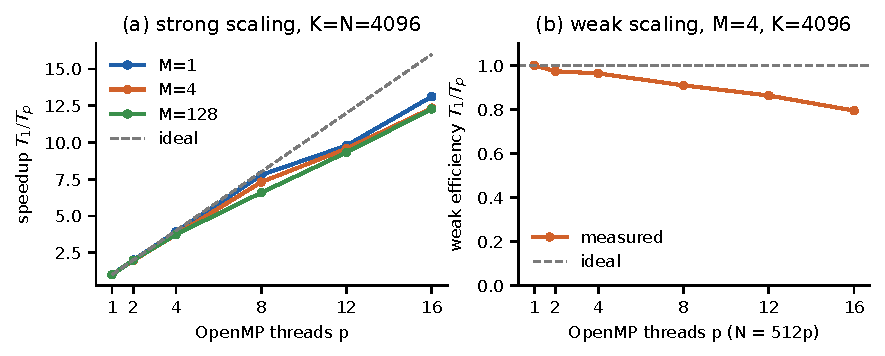
\includegraphics[width=\textwidth]{figs/e041_scaling.pdf}
\caption{CPU fused W4A16 GEMM (E041), medians of 10 runs on the 16-core EPYC~9115. (a) Strong scaling at $K=N=4096$; (b) weak scaling at $M=4$ with $N=512p$.}
\label{fig:scaling}
\end{figure*}
\begin{table}[t]
\caption{E041, same node and job: serial time $T_1$, 16-thread speedup $S_{16}=T_1/T_{16}$ and efficiency $E_{16}$, and our fastest GPU kernel of that time (no flush) and its ratio to $T_1$.}
\label{tab:e041}
\small
\setlength{\tabcolsep}{4pt}
\begin{tabular}{rrrrrlr}
\toprule
$M$ & $T_1$ (ms) & $S_{16}$ & $E_{16}$ & GPU ($\mu$s) & kernel & $T_1$/GPU \\
\midrule
1 & 26.57 & 13.12 & 0.82 & 38.4 & E001 & 691 \\
4 & 31.29 & 12.34 & 0.77 & 58.6 & E003 & 534 \\
128 & 241.24 & 12.27 & 0.77 & 1499.7 & E003 & 161 \\
\bottomrule
\end{tabular}
\end{table}

\paragraph{Result.} Fig.~\ref{fig:scaling} and Table~\ref{tab:e041} give $S_p = T_1/T_p$. $M=1$ and $M=4$ scale near-linearly to 8 threads (7.79$\times$ and 7.30$\times$); $M=128$ reaches 6.58$\times$ there. At 16 threads speedup is 12.3--13.1$\times$, and weak-scaling efficiency falls to 0.79. The hypothesis is not confirmed: $M=1$ scales best, moves only about 4.3\,GB/s of modelled weight bytes at 16 threads, and its 8.65\,MB of codes and scales fit in L3, so this CPU kernel is compute-bound. Static distribution of 64 column blocks over 12 threads gives at most 6 blocks per thread, which bounds $S_{12}$ by 10.7 (calculated); the measured 9.3--9.8$\times$ stay below that bound, and the remaining losses are unattributed (no CPU profile). Our scalar GPU kernels of that time are 161--691$\times$ faster than $T_1$ and 13--53$\times$ faster than all 16 cores; these ratios compare different processors and are not parallel speedups of one program.

\subsection{Rung 1: naive CUDA kernel}
The naive kernel assigns one thread to each output, 256 threads per block on a grid of $\lceil N/256 \rceil \times M$ blocks, and loops over all of $K$. It is the denominator of E001. Its Nsight Compute profile at $M=1$ (cache-invalidated replay) shows the problem: only 16 blocks for 36 SMs, active warps 16.6\% of peak and SM throughput 9.2\%.

\subsection{Rung 2: in-block $K$ splitting (E001)}
\emph{Evidence:} the 16-block grid above. \emph{Hypothesis:} eight threads per output, each summing a contiguous eighth of $K$ and reducing through shared memory, shorten the serial chain and multiply the block count by eight. \emph{Criterion:} median speedup $>1$ over naive at $M=1$ under both cache policies. \emph{Change:} blocks of $32\times 8$ threads, one warp per $K$ slice, a 1\,KB shared-memory reduction in fixed slice order (the FP32 addition order therefore changes). \emph{Correctness:} FP64 check and exact $\hat W$ at every point; memcheck and synccheck clean on the selected small cases. \emph{Result (Table~\ref{tab:ladder}):} 3.85$\times$ with store flush and 2.89$\times$ without; the post-change profile shows 128 blocks and active warps rising from 16.6\% to 55.5\% at nearly unchanged DRAM bytes. \emph{Limitation:} it is slower than naive at every larger $M$ (0.88/0.99 at $M=8$, 0.75--0.81 at $M=32$ and 128), where one thread per output already fills the GPU; one final series on one node.

\subsection{Rung 3: aligned-shape specialization (E002)}
\emph{Evidence:} E001 keeps a runtime final-word bounds check in its inner loop even at aligned $K=4096$; while preparing E001, the same kind of guard had measurably slowed the naive kernel. \emph{Hypothesis:} compiling separate aligned and tail versions removes that overhead. \emph{Criterion:} speedup $\ge 1.05$ over E001 at $M=32$ and 128 under both policies, with at most 5\% regression at $M=1$. \emph{Change:} a template on $K \bmod 8$ with \texttt{if constexpr} guards; mapping and arithmetic unchanged. \emph{Correctness:} every output of every main point bit-identical to E001, FP64 check, six sanitizer runs clean. \emph{Result:} 1.31--1.33$\times$ at $M=32$--128; at $M=1$ 1.04$\times$ with store flush and 1.28$\times$ without. The aligned machine code shrinks from 240 to 216 instructions and branches from 11 to 4 (static counts), and the profile shows 23.1\% fewer executed warp instructions at both $M=1$ and $M=128$ with unchanged DRAM and L2 bytes. \emph{Limitation:} one series; at $M=128$ it is still slightly slower than naive.

\subsection{Rung 4: row reuse (E003) --- the profile-to-fix chain}
\emph{Evidence:} the cache-invalidated profile of E002 at $M=128$ records 1151\,MB of L2 traffic against 9.9\,MB read from DRAM: every row reloads and re-decodes the same packed weights. \emph{Hypothesis:} decoding each weight once for two or four rows removes enough repeated work to outweigh more registers and fewer blocks. \emph{Criterion:} speedup $\ge 1.05$ over E002 at $M=32$ and 128 under both policies. \emph{Change:} each decoded $\hat w$ feeds two or four independent row accumulators; per-row arithmetic order is unchanged. \emph{Correctness:} every output bit-identical to E002 at every main point including all 128 rows at $M=128$; six sanitizer runs clean. \emph{Result:} two rows 1.55--1.57$\times$ and four rows 1.69--1.75$\times$ at $M=32$--128, in both series. After the change L2 traffic at $M=128$ is 641\,MB (two rows) and 384\,MB (four rows), 44.3\% and 66.7\% less, executed warp instructions fall 38.1\% and 57.2\%, and DRAM reads stay at 9.7\,MB: the change removed repeated on-chip work, not DRAM traffic. This is the one rung where a profile identified the cost, a single change targeted it, and the counters and the latency moved together. \emph{Limitation:} at $M=1$ there is nothing to reuse (no flush: 30.0\,$\mu$s rises to 36.4 and 58.9\,$\mu$s; four rows with store flush 63.1\,$\mu$s); at $M=5$ two rows gain 1.21$\times$/1.20$\times$, four rows gain 1.08$\times$ with store flush but are slower without it.

\subsection{Rung 5: wider operand loads (E043)}
\emph{Evidence:} no Nsight profile was taken before this rung. E041 put our best kernels at 38.4\,$\mu$s ($M=1$) and 58.6\,$\mu$s ($M=4$, four rows, no flush), against 19.3\,$\mu$s to stream the 8.67\,MB of modelled bytes at $M=1$ at 448\,GB/s; reading the source showed one 2-byte load per activation and one scale load per packed word although the eight activations are contiguous and the scale changes every 16 words. \emph{Hypothesis:} at small $M$ the scalar kernels are limited by load-instruction issue. \emph{Criterion:} median $\ge 5\%$ lower than E002 at $M=1$ and than the E003 four-row kernel at $M=4$, both policies, both series, every node. \emph{Change:} only operand fetches: one 16-byte activation load per row per packed word and one scale load per group; mapping, slices and addition order unchanged. Static global-load instruction sites per kernel function fall from 10 to 7 (one row) and from 34 to 6 (four rows). It requires $K$ divisible by 8 and 16-byte-aligned activations, otherwise it calls the parent. \emph{Correctness:} 182 full-output bitwise comparisons with the parents, zero differences; memcheck, synccheck and racecheck clean. \emph{Result:} on five nodes and in both series this is 31--33\% faster at $M=1$ (16--22\% without flush) and 18--21\% faster for the four-row kernel at $M=4$ (36--38\%), with no regression at any tested $M$ or held-out shape; with store flush, $M=1$ rises from 0.38 to 0.56 of the modelled memory roof. Up to $M=4$ our kernels are now 1.4--3.5$\times$ faster than cuBLAS on the FP16 $\hat W$ (single repeated matrix). \emph{Limitation:} from $M=32$, cuBLAS with Tensor Cores is 2.8--8.5$\times$ faster; the load counts support, but do not prove, the load-issue explanation. The later E046 profile of the four-row kernel at $M=1$ shows DRAM at 44.9\% of peak with long-scoreboard the top stall (47\% of samples).

\subsection{Rung 6: our Tensor Core kernel (E044)}
\emph{Evidence:} no Nsight profile was taken before this rung either; the evidence was E043's gap to cuBLAS from $M=32$, which we attributed, without a profile, to scalar FP32 multiply--adds and per-weight decoding rather than to weight bytes. \emph{Hypothesis:} replacing scalar multiply--adds with FP16 Tensor Core MMAs with FP32 accumulation lowers latency at $M \ge 8$. \emph{Criterion:} median $\ge 5\%$ lower than the E043 four-row kernel at $M=8$, 32 and 128, both policies, both series, every node. \emph{Change:} \texttt{mma.sync.m16n8k16} written from the PTX ISA fragment layouts~\cite{ptx}, not from Marlin's source; a block of eight warps computes a $16\times 32$ output tile, the warps split $K$ in chunks of 64 and reduce in shared memory in fixed order; rows beyond $M$ are zero. Weights are decoded two at a time with packed FP16 operations: $(1024+q) - 1032 = q-8$ exactly, then one FP16 multiply by $s$, which an exhaustive self-test over every finite FP16 scale and every code confirms gives the same bits as the contract's formula. It requires $K$ and $g$ divisible by 64, $N$ by 32 and 16-byte-aligned activations (otherwise the E043 kernel runs); its paired FP16 stores also assume 4-byte-aligned outputs, which the launcher does not check (all buffers here come from \texttt{cudaMalloc}). \emph{Correctness:} FP64 tolerance only, not bitwise, because the addition order changes; all sampled outputs pass (at $M=128$ half the rows are sampled), the unpack self-test finds 0 mismatches, sanitizers are clean. \emph{Result:} on five nodes and in both series it is 55--57\% faster at $M=8$, 80\% at $M=32$ and 85\% at $M=128$ with store flush (71--87\% without), and faster at every tested $M$ and held-out shape. The fast decode alone is worth 1.10--1.44$\times$ at $M \le 8$ and 1.00--1.12$\times$ above. Against cuBLAS (default math mode) on the FP16 $\hat W$ it is faster up to $M=64$ with store flush and 1.10--1.20$\times$ slower at $M=128$, where E043's kernel was 7.7--8.5$\times$ slower. \emph{Limitation:} the gain belongs to the whole design (MMA, tiling and operand handling changed together), not to the MMA alone; single repeated matrix.

\subsection{Against the ceiling: cyclic comparison with Marlin (E045)}
\label{sec:e045}
\emph{Question:} how close is our Tensor Core kernel (E044, source unchanged) to corrected Marlin when, as in a model, the weights do not stay in cache between uses? \emph{Hypothesis:} slower than Marlin everywhere, with the smallest gap at $M=4$ and the largest at $M=128$. \emph{Design:} E010's cyclic harness unchanged (Table~\ref{tab:protocol}): two layer shapes, four independent weight matrices each (seeds 3--6, more than the 32\,MiB L2 together), $M \in \{4,16,64,128\}$, our kernel, corrected Marlin and cuBLAS (mode 16) on pre-materialized FP16 $\hat W$ in the same process, one node (c7). \emph{Correctness:} every active row of every path within the FP64 tolerance in direct and graph-replayed cycles and again after timing; the library's four kernel bodies are instruction-identical to the E044 build; traces show exactly one kernel launch per call; memcheck and synccheck on the composed cycle and racecheck on our kernel are clean.

\begin{table*}[t]
\caption{E045: amortized time per GEMM (four-matrix cycle median$/4$) under cyclic reuse, series 1 / series 2, one node. ``Fraction'' = Marlin time / our time, i.e.\ the fraction of Marlin's speed our kernel reaches.}
\label{tab:e045}
\small
\begin{tabular}{lrrrrr}
\toprule
$K\times N$ & $M$ & ours (tc), $\mu$s & corrected Marlin, $\mu$s & cuBLAS FP16 $\hat W$, $\mu$s & fraction of Marlin speed \\
\midrule
4096$\times$11008 & 4 & 64.4 / 63.9 & 61.3 / 60.9 & 268.9 / 269.2 & 0.95 / 0.95 \\
4096$\times$11008 & 16 & 71.6 / 71.1 & 64.3 / 63.8 & 247.7 / 246.7 & 0.90 / 0.90 \\
4096$\times$11008 & 64 & 184.5 / 184.2 & 131.2 / 131.8 & 245.8 / 243.4 & 0.71 / 0.72 \\
4096$\times$11008 & 128 & 338.2 / 337.8 & 250.7 / 250.9 & 257.2 / 256.1 & 0.74 / 0.74 \\
11008$\times$4096 & 4 & 67.2 / 67.5 & 59.2 / 59.2 & 214.9 / 214.9 & 0.88 / 0.88 \\
11008$\times$4096 & 16 & 69.5 / 70.5 & 61.3 / 61.2 & 215.7 / 215.7 & 0.88 / 0.87 \\
11008$\times$4096 & 64 & 177.6 / 178.6 & 129.5 / 129.6 & 223.9 / 224.1 & 0.73 / 0.73 \\
11008$\times$4096 & 128 & 326.5 / 327.6 & 245.5 / 244.6 & 290.7 / 293.8 & 0.75 / 0.75 \\
\bottomrule
\end{tabular}
\end{table*}

\emph{Result (Table~\ref{tab:e045}):} our kernel reaches 88--95\% of corrected Marlin's speed at $M=4$, 87--90\% at $M=16$, 71--73\% at $M=64$ and 74--75\% at $M=128$. It is slower than Marlin in all 16 cell-series, but 3.1--4.2$\times$ faster than cuBLAS on the FP16 weights at $M \le 16$; at $M=128$ cuBLAS is 1.12--1.32$\times$ faster than ours. The hypothesis is not confirmed: the gap peaks at $M=64$, not $M=128$. \emph{Limitation:} one node, synthetic weights, unprofiled in this harness; offline preparation (Marlin's repack, uploading codes, materializing $\hat W$) is outside timing for every path.

\subsection{First profile of our Tensor Core kernel (E046)}
\emph{Question:} where does our Tensor Core kernel spend its time, and which single change should the next rung make? This is a diagnostic: no kernel change and no gate. \emph{Hypotheses, stated before profiling:} (a) at $M=1$ it is limited by global-load latency with poorly coalesced weight loads and DRAM below 60\% of peak; (b) at $M=128$ it is limited by every 16-row tile reloading and re-decoding all weights, with the tensor pipe below 30\% busy. \emph{Method:} Nsight Compute kernel replay of the unchanged single-matrix benchmark with cache invalidation, one node (c58).

\begin{table}[t]
\caption{E046 Nsight Compute replay counters, $K=N=4096$ (replay durations are not production latency). Waves (our kernel only) = blocks / 108 resident slots (36 SMs $\times$ 3 register-limited blocks).}
\label{tab:e046}
\small
\setlength{\tabcolsep}{3pt}
\begin{tabular}{lrrrrl}
\toprule
Kernel, $M$ & $\mu$s & DRAM \% & tensor \% & waves & top stall \\
\midrule
ours (tc), 1 & 26.2 & 75.0 & 55.8 & 1.19 & long scoreboard 63\% \\
ours (tc), 16 & 27.0 & 74.0 & 53.1 & 1.19 & long scoreboard 34\% \\
ours (tc), 128 & 132.1 & 16.7 & 82.8 & 9.48 & math pipe 33\% \\
E043 four-row, 1 & 43.7 & 44.9 & 0.0 & -- & long scoreboard 47\% \\
cuBLAS, 1 & 84.5 & 94.0 & 0.0 & -- & long scoreboard 32\% \\
cuBLAS, 128 & 112.7 & 72.8 & 96.9 & -- & math pipe 61\% \\
\bottomrule
\end{tabular}
\end{table}

\emph{Result (Table~\ref{tab:e046}):} both hypotheses are rejected. At $M=1$ long-scoreboard waits dominate the samples, as predicted, but DRAM is already at 75\% of peak and every 32-byte sector the weight loads fetch is fully used. At $M=128$ weight traffic through L2 is indeed eight times the code bytes, but the tensor pipe is 83\% busy and executes exactly cuBLAS's 1,048,576 MMA instructions in the same tensor-pipe busy time (109\,$\mu$s), and activation re-reads exceed weight re-reads in L2. The clearest inefficiency is at small $M$: 128 blocks fill only 1.19 waves of the 108 resident slots, and the SMs are active on average 82\% of the elapsed cycles (the least busy 69\%). The same weight bytes on the $4096\times11008$ shape, at 3.19 waves, reach 84\% of DRAM peak. \emph{Limitation:} replay with a cold cache on one repeated matrix is neither the cyclic regime of Table~\ref{tab:e045} nor production latency; the link from waves to latency is an inference from counters and a two-shape comparison.

\emph{Recommendation for the next rungs:} first fill the GPU at small $M$ by splitting $K$ across blocks with a fixed-order reduction (expected about 10\% at $M \le 16$); second, a 32-row tile at large $M$, which the counters bound at about 17\% at $M=128$ because it cannot reduce the MMA count; repacking or deeper prefetching is not supported until the first is measured.

\subsection{Rung 7: split-$K$ at small $M$ (E047)}
\emph{Evidence:} E046 (Table~\ref{tab:e046}): at $M \le 16$ our kernel's 128 blocks fill 1.19 waves, and the same weight bytes at 3.19 waves reach a higher DRAM fraction. \emph{Hypothesis:} splitting $K$ across blocks raises the small-$M$ grid to several waves and lowers latency by about 10\% at $M \le 16$. \emph{Criterion:} median $\ge 5\%$ lower than E044's kernel at $M=1$, 4 and 16, both policies, both series, every node. \emph{Change:} each $16\times32$ output tile gets four blocks that each take a quarter of $K$, with E044's warps, fragments and decode unchanged; each block writes its FP32 partial tile to a global workspace and the last block to arrive sums the four in fixed order, inside the same launch. A fixed rule splits only below three waves of resident blocks; otherwise E044's kernel runs. \emph{Correctness:} every output row of every timed point is within the FP64 tolerance (not bitwise, because the addition order changes), a second launch matches the first bit for bit, and the sanitizers are clean. \emph{Result:} rejected, 0 of 60 primary cells. It is slower than its parent in every primary cell: 26--42\% with store flush and 10--24\% without at $M=1$--16 (Table~\ref{tab:ladder}). The only gain is on the held-out $11008\times4096$ shape at $M=32$ with store flush (12--13\%). \emph{Limitation:} unprofiled; the cause is a hypothesis. With a quarter of $K$ each warp keeps only two 64-wide chunks, and the compiled split kernel holds 16 MMA instructions against the parent's 32 (a one-chunk instead of a two-chunk loop body), so fewer loads may be in flight; the reduction and its workspace may also cost time. Single repeated matrix.

\subsection{Rung 8: 32-row tile at large $M$ (E048)}
\emph{Evidence:} E046: at $M=128$ every 16-row tile reloads and re-decodes every weight, but the tensor pipe is already 83\% busy, which bounds the gain at about 17\%. \emph{Hypothesis:} a 32-row tile in which each warp's two 16-row MMA tiles share every decoded weight fragment halves weight loads and decoding per output row and lowers latency at $M \ge 32$. \emph{Criterion:} median $\ge 5\%$ lower than E044's kernel at $M=32$, 64 and 128, both policies, both series, every node. \emph{Change:} only the tile height; $M<32$ calls the parent unchanged. \emph{Correctness:} each 16-row tile receives the same MMA sequence and reduction order, so every output must match the parent bit for bit; it does at every timed point, every row also passes FP64, and the sanitizers are clean. \emph{Result:} rejected, 35 of 60 primary cells. At $M=128$ it is 4.5--10.2\% faster (17 of 20 cells pass), and 4.3--20.1\% faster on the held-out rectangles at $M \ge 32$; but with store flush it is 8--13\% slower at $M=32$ and ties at $M=64$ ($-2.7$ to $+0.5\%$). At $M=128$ with store flush it narrows the gap to cuBLAS (default math mode) from 1.18--1.19$\times$ to 1.10--1.13$\times$. \emph{Limitation:} unprofiled. The kernel needs 114 registers per thread against the parent's 64--76, so 2 instead of 3 blocks fit per SM, and at $K=N=4096$, $M=32$ the grid has only 128 blocks; we hypothesize that lost occupancy outweighs the saved loads on small grids. A dispatch by $M$ or grid size chosen from these data would be post hoc and is not claimed. Single repeated matrix, not comparable with Section~\ref{sec:e045}.

\subsection{Why Marlin is faster at $M \ge 64$: cyclic profile (E049)}
\label{sec:e049}
\emph{Question:} under weight cycling our kernel's gap to Marlin peaks at $M=64$ (Table~\ref{tab:e045}), but E046 profiled only one repeated matrix. This is a diagnostic: no kernel change and no gate. \emph{Hypotheses, with verdict rules fixed before profiling:} (a) at $M=64$ the four 16-row tiles re-read the weights from DRAM (rejected if our DRAM reads stay below 1.2 times the unique operand bytes $U$); (b) Marlin's asynchronous-copy pipeline hides load latency that ours exposes (confirmed if our long-scoreboard stall share is $\ge 30\%$ and at least twice Marlin's); (c) every 16-row tile repeats each weight load and decode (confirmed if we execute $\ge 1.5\times$ Marlin's warp instructions with issue active $\ge 40\%$). \emph{Method:} Nsight Compute application replay inside E045's four-matrix cycle, profiling the last GEMM of the 100th graph-replayed cycle so that every pass sees the real preceding accesses, without profiler flush; 18 passes per case, each with outputs equal to its validated outputs; one node (c8).

\begin{table}[t]
\caption{E049 replay counters under cyclic weights (replay durations are not production latency). DRAM$/U$ = DRAM read bytes over unique operand bytes; LSB = long-scoreboard share of stalls.}
\label{tab:e049}
\small
\setlength{\tabcolsep}{3pt}
\begin{tabular}{lrrrrrr}
\toprule
Kernel, $M$ & $\mu$s & DRAM$/U$ & DRAM \% & tensor \% & inst (M) & LSB \% \\
\midrule
\multicolumn{7}{l}{$K\times N=$ 4096$\times$11008} \\
ours (tc), 4 & 66.1 & 1.00 & 80.1 & 51.1 & 8.10 & 47 \\
Marlin, 4 & 62.4 & 1.00 & 85.1 & 27.2 & 3.61 & 26 \\
ours (tc), 64 & 196.4 & 0.94 & 28.7 & 70.7 & 29.15 & 24 \\
Marlin, 64 & 137.8 & 0.93 & 43.5 & 90.8 & 5.61 & 2 \\
\multicolumn{7}{l}{$K\times N=$ 11008$\times$4096} \\
ours (tc), 4 & 75.2 & 1.00 & 70.3 & 52.9 & 7.95 & 53 \\
Marlin, 4 & 60.3 & 1.00 & 88.2 & 26.6 & 3.54 & 39 \\
ours (tc), 64 & 193.0 & 0.96 & 29.0 & 75.0 & 28.15 & 25 \\
Marlin, 64 & 136.1 & 0.93 & 41.6 & 91.5 & 5.46 & 2 \\
\bottomrule
\end{tabular}
\end{table}

\emph{Verdicts (Table~\ref{tab:e049}, the same on both rectangles):} (a) rejected: at $M=64$ we read 0.94--0.96\,$U$ from DRAM (Marlin 0.93\,$U$); the tiles' re-reads hit L2 (91.3--91.5\% of SM reads), and the extra DRAM bytes explain 0.8--3.4\% of the profiled gap. (b) partial: our long-scoreboard share of 24--25\% is more than ten times Marlin's 2\%, but below the 30\% bar and level with load-store and math-pipe throttling. (c) confirmed: both kernels execute the same 1,409,024 MMA instructions, but we issue 5.2$\times$ Marlin's warp instructions (19.0--19.7 against 2.9--3.0 other instructions per MMA) at 41--43\% issue active. Occupancy is not the limiter: we keep 48--49\% of warp slots resident against Marlin's 17\%. Marlin is tensor-pipe bound (91--92\% busy, math-pipe throttle 67\% of stalls); ours is 71--75\% busy. At $M=4$ both read $U$ once and are DRAM-bound (ours at 70--80\%, Marlin at 85--88\% of peak), and on $11008\times4096$ our 128 blocks fill only 1.19 waves.

\emph{What it implies:} the remaining gap at $M \ge 64$ is instruction overhead from reloading and re-decoding the weights in every 16-row tile, not DRAM traffic. In the same job, re-timed in the cycle, our kernel, Marlin and cuBLAS reproduce E045's medians within 1\%, and E048's 32-row tile, which shares each decoded weight between two tiles, reaches 0.83--0.86 of Marlin's speed at $M=64$ and 0.87 at $M=128$ (ours: 0.71--0.75), 12.5--17.3\% faster than our kernel there with bitwise-equal outputs. This is descriptive, not an accepted rung: E048 was rejected and a threshold at $M \ge 64$ would be chosen from these data. The recommended next rung, E050, dispatches the 32-row tile at $M \ge 64$ with a 5\% criterion against our kernel, on fresh weight seeds because the threshold is post hoc; it has not been run. \emph{Limitation:} one node; replay counters of one fixed operation; stall shares are warp-state ratios, not time.

\section{Marlin as the ceiling, and the roofline}
\label{sec:ceiling}
\paragraph{Integration and the race fix (E004--E006).} We call Marlin's dense 4-bit operator directly with our codes and scales. While testing an alternative launch setting (E005), Compute Sanitizer's racecheck~\cite{sanitizer} reported shared-memory hazards in all tested configurations and in the isolated official vLLM wheel, so E005 stopped at that safety gate with no timings released. We traced the hazard to a shared buffer reused for the final reduction while other warps could still read it, and added one block barrier after the existing asynchronous-copy drain in the pinned source (E006). In the tested configurations this removes the reported hazard, and the corrected kernel passes the full numerical checks and representative memcheck, racecheck and synccheck runs. This is bounded evidence: it is not a general validation of other formats or GPUs, the official wheel's exact source mapping was not established, and we could not show that the original kernel ever produced a wrong output. ``Marlin'' below means this corrected kernel with its original dispatch (``A'').

\paragraph{Compressed versus FP16 execution (E009, E010).} The cyclic harness is a synthetic workload with a long weight-reuse distance: its active weight set exceeds L2 capacity, though we did not measure eviction. With four matrices at $M=4$, corrected Marlin is 3.62--4.40$\times$ faster than cuBLAS on pre-materialized FP16 $\hat W$, and 8.05--9.33$\times$ faster than reconstructing $\hat W$ on the GPU and then calling cuBLAS (both series, both shapes). The lead narrows as $M$ grows without reversing up to 128: at $M=128$ it is 2.2--2.9\% for $K=4096,N=11008$ (below our 5\% bar) and 15.2--16.8\% for the transpose.

\begin{figure}[t]
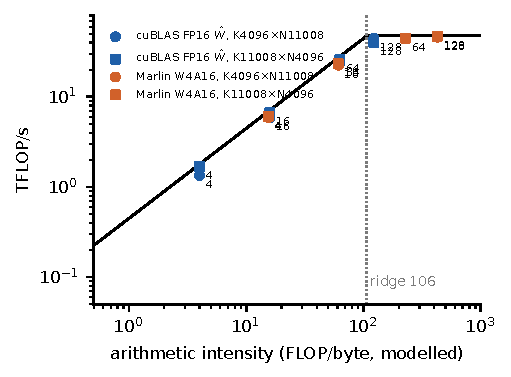
\includegraphics[width=\linewidth]{figs/roofline.pdf}
\caption{Roofline of the RTX~5060~Ti with E045's amortized per-GEMM times (series 1, one job and node): our Tensor Core kernel, corrected Marlin and cuBLAS on FP16 $\hat W$, labelled by $M$; our kernel shares Marlin's intensity. Bandwidth roof 448\,GB/s; compute roof 47.4\,TFLOP/s dense FP16 Tensor with FP32 accumulation (36 SMs $\times$ 2.572\,GHz nominal boost $\times$ 512 FLOP/clock/SM, from a third-party listing), ridge 106 FLOP/byte. Intensity uses modelled bytes, not measured DRAM traffic.}
\label{fig:roofline}
\end{figure}

\paragraph{Roofline.} Fig.~\ref{fig:roofline} places all three paths of E045. The useful work is $2MNK$ FLOP; the modelled bytes count each operand once: $KN/2$ bytes of codes plus $2NK/128$ bytes of scales (or $2KN$ bytes of FP16 $\hat W$ for cuBLAS), plus $2MK$ bytes of activations and $2MN$ of outputs, excluding cache reloads and Marlin's workspace. The compute roof assumes the nominal boost clock; the GPU ran at 2797--2805\,MHz after each E045 series, so the true compute roof is somewhat higher and the compute-side fractions below are upper estimates. At $M=4$, cuBLAS sits at 4.0 FLOP/byte and Marlin at 15.4, both left of the ridge, at 75--94\% and 85--88\% of the memory roof respectively; our kernel shares Marlin's intensity and reaches 77--82\%. For memory-bound points the speedup decomposes as $S = (I_Q/I_R)\,(\eta_Q/\eta_R)$, with $I$ the intensity and $\eta$ the fraction of the memory roof achieved; the intensity ratio is 3.9. In achieved FLOP/s, Marlin at $M=4$ (5.89--6.10\,TFLOP/s) matches cuBLAS at $M=16$ (5.83--6.69\,TFLOP/s), a statement about throughput, not about latency at equal work. At $M=64$--128 Marlin (229--426 FLOP/byte) is right of the ridge at 92--100\% of the nominal compute roof, cuBLAS at $M=128$ (123 FLOP/byte) at 83--95\%, and our kernel at 66--75\%. No point exceeds either roof. The model is consistent with the measured narrowing of Marlin's lead over cuBLAS at large $M$ and with our kernel's larger gap there, but a byte-model roofline does not attribute the critical path, and it does not explain why the transpose keeps a 15--17\% Marlin advantage at $M=128$.

\paragraph{Comparator history.} These experiments tuned or analyzed Marlin, not our kernels; they are not rungs. Three tuning attempts failed the 5\% criterion: a different shared-memory reservation and grid (E005-R1, 0--2.8\%), skipping loads never used at small $M$ (E007: shared loads fell 1.9\% but instructions rose 1.8\%), and a smaller tile at $M=128$ (E013, 7.6--8.7\% slower). A fourth (E005-R2) passed its rectangular confirmation without cache flush but regressed under store flush. That configuration's advantage on one repeated matrix (13.4\% for $4096\times11008$) did not survive cycling four matrices (1.3--2.4\%, and a 0.4--0.8\% loss on the transpose, E008); the precise cache mechanism remains unresolved. Endpoint profiles (E011) showed nearly constant DRAM bytes with more instruction and Tensor work at $M=128$; source-level PC sampling (E012) failed its own data-quality checks, so no code-region attribution was made and Marlin was not rewritten. Marlin stays the ceiling; we did not move it.

\section{Background: the model-level study (E014--E042)}
\label{sec:model}
This frozen study motivated the small-$M$ regime. We replaced all 196 block projections of Qwen2.5-1.5B~\cite{qwen25} with corrected Marlin (batch 1, greedy, 64 tokens, one GPU type). None of our own kernels is in that path.

\paragraph{Validation.} The GEMM tolerance does not apply to whole models. Two predeclared gates against the FP16 model on the same reconstructed weights rejected the path: E017 (591 of 9,723,904 logits outside an elementwise bound, all 64 tokens identical) and E019 (the FP16 reference lost an exact FP16 tie in one case; another case missed one criterion by 0.000003). E018 found zero failures over 196 modules $\times$ 64 forwards of same-input operator calls, and Marlin-free FP32/FP64 controls failed the same bound, so we interpret the E017 difference as propagated FP16 rounding, for that one context-128 request. A third gate, agreement with an FP64-projection control (E021), accepted all ten cases. It was chosen after the first two failed; four of its ten cases were known beforehand, six were fresh contexts 256/512/1024, and there is no sanitizer coverage at those prefill sizes. E017 and E019 remain failed. Every model speedup below holds only under this third gate and was measured with plain-rounded 4-bit blocks that cost 13.1\% WikiText-2~\cite{wikitext} perplexity over the FP16 original (E032; the FP16 baselines used the same reconstructed weights).

\paragraph{Speed.} Eager Marlin decoded 28.9--29.0\% faster than FP16 at context 2048 but only 3.6--4.6\% at 128 (E020). In an isolated sequence of the 196 projections, Marlin calls were 99\% host time (E022); that the whole step was host-bound is a hypothesis, supported at short context by CUDA-graph replay~\cite{cudagraphs} (E023), which is bitwise equal to eager Marlin and 42--43\% faster than it at context 128 (passes) but 2\% at 2048 (misses). E024 found graph-replayed Marlin's gain over FP16 (before the attention change) robust in 28 cells on two nodes. A direct single-query decode attention (E026) then gives about 325 and 374\,ms per 63 tokens at contexts 128 and 2048, 45.4--45.5\%/42.5\% below graph-replayed FP16 with the same attention and 47.0--47.1\%/58.5\% below graph-replayed FP16 with stock attention; the attention change itself is about 5\% at context 128, below the bar in two of eight cells, and is not a default.

\paragraph{External stacks.} Our path is slower than vLLM: on the identical codes and scales vLLM v0.33.0 (unpatched Marlin, its own runtime) decodes in 238.1--248.9\,ms against our 326.8--376.0\,ms, 37--51\% slower at contexts 128--2048 (E027). llama.cpp~\cite{llamacpp} and ONNX Runtime GenAI~\cite{ortgenai} are faster still; that comparison is stack against stack, since they use their own quantizers, quantize the embedding/output matrix too, and their quality was not measured. A trace (E030) shows a per-step device-time gap of 1.4--2.0\,ms, about 0.4\,ms of it inside Marlin projections; vLLM issues 112 Marlin calls per step against our 196 and over four times fewer other kernel launches. These differences accompany its lower device time; they do not isolate the cause. A 4-bit output head lowers our decode time by 17.0\%/14.7\% at contexts 128/2048 (E031) but changes model outputs and costs a further 8.6\% perplexity (E032), and our path with it is still slower than stock vLLM.

\paragraph{Quality.} A GPTQ-style~\cite{gptq} quantizer of our own in the same format, calibrated on C4~\cite{c4}, lowers the block cost to 5.62\% (E037), still failing a 5\% bar. Ten variants were scored on the test split and three were added after a test table had been seen; the selection used the validation split only. E038 gated and timed that checkpoint: decode within 0.3\% of the plain-rounded weights for its four arms at contexts 128/2048 on one node; no FP16 baseline was timed on it. Upstream llm-compressor~\cite{llmcompressor} GPTQ costs 5.15\% and our implementation on the standard 16-level grid 5.27\% (E039), so ours matches upstream and the grid has no material effect; the 16-level arms are quality-only, outside our runtime format. AWQ~\cite{awq} costs 5.72--10.21\% across three tested recipes (E040; one asymmetric, outside our format), so it does not help here; all arms fail the 5\% bar. The cost is spread across layers rather than concentrated (E042). These bound one 1.5B model, one corpus and one metric; other recipes and larger models are untested.

\section{Failures and lessons}
\begin{itemize}
\item \textbf{Profile before choosing.} Only E003 followed a profile directly to a fix that both counters and latency confirmed. E043 and E044 succeeded without a prior profile, and the first profile of our Tensor Core kernel (E046) rejected both of our explanations for its remaining gap; the two rungs it then selected (E047, E048) were both rejected, so a profile narrows the choice without guaranteeing the fix. Profiling in the regime that matters helps: the cyclic profile (E049) located the gap that the single-matrix profile missed.
\item \textbf{A gain on one shape is not a gain.} E001 is 3.85$\times$ faster at $M=1$ and slower at every larger $M$; row reuse loses at $M=1$; the gap to Marlin peaks at $M=64$, not where we predicted.
\item \textbf{Single-matrix benchmarks can mislead.} A 13\% Marlin launch-setting gain on one repeated matrix fell below 5\% when matrices were cycled (E008), which is why the ladder is compared with Marlin only in the cyclic harness.
\item \textbf{Check the tools.} Marlin's race (E005/E006), \texttt{mpirun} pinning all OpenMP threads to one core (E041, caught by a guard before any timing), and a profiler that wrote a different report extension and metric names than expected (E046) were all found by checking preconditions instead of trusting outputs.
\item \textbf{Fix the gate before timing.} At model level two numerical gates failed (E017, E019), and the accepted speedups carry the disclosure that their gate came third.
\end{itemize}

\section{Conclusion}
Our own ladder climbed from a 16-core CPU baseline through scalar fused kernels (in-block $K$ splitting, specialization, profile-guided row reuse, wider loads) to a Tensor Core kernel that is 55--87\% faster than the best scalar kernel at $M=8$--128 on one repeated matrix. Under weight cycling it reaches 88--95\% of corrected Marlin's speed at $M=4$ and 71--75\% at $M \ge 64$, and it is slower than Marlin in every measured cell. Its first profile rules out uncoalesced loading at small $M$, where DRAM is at 75\% of peak and the clearest remaining inefficiency is an under-filled grid (an inference that E047 did not bear out), and shows the large-$M$ kernel already tensor-pipe bound. The two rungs it selected were both rejected under their 5\% criteria: split-$K$ is slower in every primary cell, and a 32-row tile wins at $M=128$ but loses at $M=32$ with store flush. Our Tensor Core kernel (E044) therefore remains our best. A cyclic profile against Marlin (E049) shows that the remaining gap at $M \ge 64$ is instruction overhead from reloading and re-decoding the weights in every 16-row tile (5.2$\times$ Marlin's instructions for the same MMAs), not DRAM traffic; the recommended next rung, dispatching the 32-row tile at $M \ge 64$ on fresh weight seeds (E050), has not been run. None of our kernels is in the model path, where the measured model speedups belong to upstream Marlin under a post hoc gate. Limitations: one GPU type, synthetic weights at kernel level, one model at model level, an untuned CPU baseline.

\paragraph{Artifacts.} The repository holds the code, scripts, per-experiment records and the raw results that fit in git. Ten raw files over GitHub's 100\,MB limit are kept outside git with their SHA-256 hashes recorded, and model checkpoints and logit archives remain on the cluster's scratch storage with hashes recorded in \texttt{results/}; the authors can provide them on request. The kernels are CUDA C++; Python drives the model-level measurements and analysis.

\appendix
\section{Experiment index}
\begin{table*}[t]
\small
\begin{tabular}{p{0.15\textwidth}p{0.18\textwidth}p{0.56\textwidth}}
\toprule
Experiment & Kind & Outcome \\
\midrule
E041 & CPU baseline & Descriptive; both correctness criteria met; bandwidth hypothesis not confirmed. \\
E001 & our kernel, latency & Accepted at $M=1$ (3.85$\times$); slower at larger $M$. \\
E002 & our kernel, latency & Accepted (1.31--1.33$\times$ at $M=32$--128). \\
E003 & our kernel, latency & Accepted at $M=32$--128 (two and four rows); regressions at $M=1$, mixed at $M=5$. \\
E043 & our kernel, latency & Accepted, 40/40 primary cells on five nodes. \\
E044 & our kernel, latency & Accepted, 60/60 primary cells on five nodes. \\
E045 & our kernel vs Marlin & Descriptive: 71--95\% of Marlin's speed; ordering hypothesis not confirmed. \\
E046 & our kernel, diagnostic & Both hypotheses rejected; recommends E047. \\
E047 & our kernel, latency & Rejected, 0/60 primary cells; slower in every one. \\
E048 & our kernel, latency & Rejected, 35/60 primary cells; faster at $M=128$, slower at $M=32$ with store flush. \\
E049 & our kernel vs Marlin, diagnostic & Diagnostic: DRAM re-reads rejected, exposed latency partial, per-tile instruction overhead confirmed (5.2$\times$ Marlin's instructions at $M=64$); recommends E050 (not run). \\
E004 & Marlin integration & Diagnostic comparison; lossless repack verified. \\
E005 & Marlin, safety & Stopped at failed racecheck gate; no timings released. \\
E006 & Marlin, safety & One-barrier correction removes the reported hazard in the tested configurations. \\
E005-R1, E007, E013 & Marlin tuning, latency & Rejected (below 5\% or slower). \\
E005-R2 & Marlin tuning, latency & Rectangular confirmation passed without flush; store-flush regression. \\
E008--E010 & Marlin, characterization & Reuse distance (gain reuse-dependent); cyclic baselines (all 36 rows pass 5\%); batch crossover (no reversal to $M=128$). \\
E011, E012 & Marlin, diagnostic & Profiles; PC sampling failed its quality checks. No change justified. \\
E014--E016 & model FP16 graphs & E014 stopped at its numerical gate; E015/E016 below 5\%. \\
E017, E019 & model gate & Failed (Marlin path rejected against FP16). \\
E018 & model, diagnostic & Interpretation: propagated FP16 rounding, one request. \\
E020 & model, descriptive timing & Measured on a path that had failed E017/E019. \\
E021 & model gate & Third gate, accepted in all ten cases (post hoc). \\
E022, E025, E030 & model, diagnostic & Host-bound projections; attention cost; gap to vLLM located on the device. \\
E023 & model, latency & Passes at context 128, misses at 2048. \\
E024 & model, robustness & All 28 cells pass. \\
E026 & model, latency & Passes at 256--2048; about 5\% at 128, below the bar in two of eight cells. \\
E027--E029 & model, external & Ours slower than vLLM, llama.cpp and ONNX Runtime GenAI. \\
E031, E033, E035 & model, latency & Quantized heads faster; they change outputs; E035 vLLM only, no logit gate. \\
E032, E034 & model, quality & Blocks +13.1\%, 4-bit head +8.6\%; no uncalibrated 4-bit head within 5\%. \\
E036--E040 & model, quality & Calibrated heads pass; block cost fails 5\% in every recipe; E038 equal speed for its arms. \\
E042 & model, quality diagnostic & Cost spread across layers; concentration hypothesis not confirmed. \\
\bottomrule
\end{tabular}
\end{table*}

\bibliographystyle{ACM-Reference-Format}
\bibliography{references}
\end{document}
